%==========================================================================================
%
%								Uniwersytet Zielonogórski
%
%						SZABLON PRACY DYPLOMOWEJ W~PAKIECIE LaTeX
%							wykonany podczas zajęć seminarjnych
%				pod przewodnictwem prof. dr hab. inż Dariusza Ucińskiego
%
%							 Damian Kowalów, Mariusz Buciakowski
%
% 				       Wydział Informatyki, Elektrotechniki i Automatyki
%						Instytut Sterowania i~Systemów Informatycznych
%
%							 Zielona Góra, kwiecień 2013
%			   (ostatnia modyfikacja: 01.02.2017 przez Mariusz Buciakowski)
%==========================================================================================
%\documentclass[a4paper,12pt]{book}
\documentclass[a4paper,12pt,openany]{book}
% ------------------------------------------------------------------------
% pakiet do wzorów ams
% ------------------------------------------------------------------------
\usepackage{amsmath}
\usepackage{amssymb}

% ------------------------------------------------------------------------
% język polski
% ------------------------------------------------------------------------
\usepackage[MeX]{polski}
\usepackage[utf8]{inputenc}

% ------------------------------------------------------------------------
% obsługa pdf
% ------------------------------------------------------------------------
\usepackage[pdftex,usenames,dvipsnames]{color}	%obsługa kolorów

% ------------------------------------------------------------------------
% wstawienie danych o autorze i pracy 
% ------------------------------------------------------------------------
\usepackage[pdftex,
				pagebackref=false,						% referencje w spisie literatury do strony na, której została urzyta
				draft=false,								% draft
				pdfpagelabels=false,						%
				pdfstartview=FitV,						% lub FitH
				pdfstartpage=1,							% 
				bookmarks=true,							% zakładki w pliku pdf
				pdfauthor={Autor},						% należy wpisać autora pracy
				pdftitle={Praca inżynierska},			% 
				pdfsubject={Tytuł pracy},				% tytuł
				pdfkeywords={slowa kluczowe},			% słowa kluczowe
				unicode=true]{hyperref}   


% ------------------------------------------------------------------------
%	style
% ------------------------------------------------------------------------
\usepackage{extsizes}							%więcej rozmiarów czcionek
\usepackage[a4paper,left=3.5cm,right=2.5cm,top=2.5cm,bottom=2.5cm]{geometry}
\usepackage{tocloft}								% format spisu treści
\usepackage{array}								% lepiej wyglądające tabelki
\usepackage[format=hang,
				labelsep=period,
				labelfont={bf,small},
				textfont=small]{caption}		% formatuje podpisy pod rysunkami i tabelami
\usepackage{floatflt}							% ładniejsze opisywanie obrazków tekstem
\usepackage{subfig}								% możliwość wstawiania figur w kolumnach
\usepackage{graphicx}							% do obsługi grafiki
\usepackage{here}									% wymuszanie położenia figury w danym miejscu
\usepackage{url}									% adresy internetowe
\usepackage{enumerate}							% modyfikowanie list wyliczeniowych np \begin{enumerate}[(a)]...
\usepackage{multirow}							% do tabel 
% ------------------------------------------------------------------------
% listingi
% ------------------------------------------------------------------------
\usepackage{listings}							% do wstawiania listingów programów




\usepackage{slantsc} % Pochyłe kapitaliki  np. \textsl{\textsc{Automatyka i robotyka}}

% ------------------------------------------------------------------------
% inne
% ------------------------------------------------------------------------
\usepackage{glossaries}

\usepackage{dashrule}
\usepackage{fancyhdr} 							% do stopki i nagłówka
\usepackage{calc}
\usepackage{packages/zmienne}					% zmienne dodatkowe używane min. w karcie pracy oświadczeniu i stronie tytułowej zebrane w jednym miejscu
\usepackage{packages/strona_tytulowa}
\usepackage{packages/oswiadczenie}
\usepackage{packages/karta_pracy}
\usepackage{packages/pusta_strona}
\usepackage{packages/wspolrealizacja}
\usepackage{longtable}							% do podziału tabel na wiele stron

\usepackage{indentfirst}

% ------------------------------------------------------------------------
% kodowanie czcionek
% ------------------------------------------------------------------------
\usepackage[T1]{fontenc}
\usepackage{lmodern}\normalfont %to load T1lmr.fd 

% ------------------------------------------------------------------------
% do algorytmów
% ------------------------------------------------------------------------

\usepackage{algorithm}
\usepackage{algorithmic}
\floatname{algorithm}{Algorytm}

% ------------------------------------------------------------------------
% do nomenklatury
% ------------------------------------------------------------------------

\usepackage[section]{placeins}
\usepackage{nomencl}
\makenomenclature
\usepackage{makeidx}
\makeindex
\renewcommand{\nomname}{Spis ważniejszych symboli}
% na końcu pliku z nomenklaturą należy umieścić polecenie
% \printnomenclature
% plik należy dodać poleceniem \input
%% przykład treści pliku
%% \nomenclature{$\oplus$}{Dylatacja zbioru}
%% \printnomenclature




% ------------------------------------------------------------------------
%   Kropki po numerach sekcji, podsekcji, itd.
%   Np. 1.2. Tytuł podrozdziału
% ------------------------------------------------------------------------
\makeatletter
    \def\numberline#1{\hb@xt@\@tempdima{#1.\hfil}}                      %kropki w spisie treści
    \renewcommand*\@seccntformat[1]{\csname the#1\endcsname.\enspace}   %kropki w treści dokumentu
\makeatother

\makeatother
% ------------------------------------------------------------------------
% Definicje
% ------------------------------------------------------------------------
\def\nonumsection#1{%
    \section*{#1}%
    \addcontentsline{toc}{section}{#1}%
    }
\def\nonumsubsection#1{%
    \subsection*{#1}%
    \addcontentsline{toc}{subsection}{#1}%
    }
\reversemarginpar %umieszcza notki po lewej stronie, czyli tam gdzie jest więcej miejsca
\def\notka#1{%
    \marginpar{\footnotesize{#1}}%
    }
%\def\mathcal#1{%
%    \mathscr{#1}%
%    }

\newcommand{\myemptypage}{ \newpage  \thispagestyle{empty}~\newpage}

%-------------------------------------------------------------------------
% listingi
%-------------------------------------------------------------------------
\lstdefinestyle{praca}{basicstyle=\scriptsize\ttfamily, 
								keywordstyle=\color{black}\bfseries,
								numbers=left, 
								stepnumber=1, 
								numberstyle=\tiny, 
								numbersep=10pt,
								extendedchars=true, 
								frame=tb}
\lstset{style=praca}

%-------------------------------------------------------------------------
% stopka i nagłówek
%-------------------------------------------------------------------------
\setlength{\headheight}{15pt}

\pagestyle{fancy}
\renewcommand{\chaptermark}[1]{\markboth{#1}{}}
\renewcommand{\sectionmark}[1]{\markright{#1}{}}

\fancyhf{}
\fancyhead[LE,RO]{\thepage}
\fancyhead[RE]{\textit{\nouppercase{\leftmark}}}
\fancyhead[LO]{\textit{\nouppercase{\rightmark}}}

\fancypagestyle{plain}{ %
\fancyhf{}
\renewcommand{\headrulewidth}{0pt}
\renewcommand{\footrulewidth}{0pt}}

% ------------------------------------------------------------------------
% Inne
% ------------------------------------------------------------------------
\frenchspacing
\setlength{\parskip}{3pt}           	%odstęp pomiędzy akapitami
%\linespread{1.49}                    	%odstęp pomiędzy liniami (interlinia)
\setcounter{tocdepth}{3}
\setcounter{secnumdepth}{3}


% ------------------------------------------------------------------------
% Polskie podpisy
% ------------------------------------------------------------------------
\renewcommand{\figurename}{Rys.}
\renewcommand{\tablename}{Tab.}

% ------------------------------------------------------------------------
% Bibliografia
% ------------------------------------------------------------------------
\bibliographystyle{unsrt}					% kolejność według użycia
%\bibliographystyle{plain}					% kolejność alfabetyczna
  
  

%==========================================================================================
% Deklaracja fontow kapitalikowych z kodowaniem T1
%==========================================================================================
\DeclareFontShape{T1}{lmr}{bx}{sc} { <-> ssub * cmr/bx/sc }{}
\DeclareFontShape{T1}{lmr}{bx}{scit}{<-> ssub * cmr/bx/scsl}{}
%==========================================================================================
% Inne deklaracje
%==========================================================================================


%==========================================================================================
% Dane na temat pracy do wypełnienia
%==========================================================================================
\author{Kamil Majewski}
\kierunek{Informatyka}
\grupa{32INF-SSI-NP}
\title{Proceduralne generowanie terenu za pomocą algorytmu Marching Cubes}
\tytulAngielski{Procedural terrain generation using the Marching Cubes}
\uczelnia{Uniwersytet Zielonogórski}
\wydzial{Wydział Informatyki, Elektrotechniki i Automatyki}
\praca{Praca dyplomowa}
\promotor{dr inż. Marek Sawerwain}
\konsultant{}
\miasto{Zielona Góra}
\miesiac{miesiąc }	% miesiąc złożenia pracy
\rok{rok}
\dzien{dd} 			% dzień podpisania oświadczenia (cyfrowo) np. 10
\mm{mm} 				% miesiąc podpisania oświadczenia (cyfrowo) np. 01 (styczeń)

%==========================================================================================
% Uwaga! polecenie \myemptypage dodaje pustą stronę do treści. Praca oddana do dziekanatu powinna być zbudowana zgodnie z~szablonem znajdującym się na stronie WEIT (z jedną stroną pustą następującą po karcie pracy), jednak jeżeli student planuje wydruk dla siebie, zalecane jest zastąpienie poleceń \newpage poleceniem \myemptypage. Skutkuje to utworzeniem bardziej przejrzystego układu zgodnego z~zaleceniami pisania książek, czyli rozpoczynanie nowych treści na prawej stronie.
%==========================================================================================


%==========================================================================================
% Dokument główny
%==========================================================================================
\begin{document}
\pagenumbering{roman}

%=========================================================================================
% Strona tytułowa
%=========================================================================================
\thispagestyle{empty}
\stronatytulowa

\thispagestyle{empty}
\pustastrona
\newpage

%========================================================================================
% Streszczenie
%========================================================================================
\normalsize

\subsection*{Streszczenie}

Streszczenie pracy dyplomowej powinno zawierać kilkuzdaniowe omówienie zagadnień poruszanych w pracy. W tej części  należy pokrótce scharakteryzować cel oraz podstawowe założenia pracy na tle stanu nauki i techniki w danej dziedzinie, jak również zamieścić od 2 do 6 słów kluczowych.



\vspace{1cm}
\noindent\textbf{Słowa kluczowe:} praca dyplomowa, skład komputerowy, formatowanie dokumentu.
\newpage
%\myemptypage

%========================================================================================
% Spis treści, spis tabel i~rysunków
%========================================================================================
%spis treści
	\tableofcontents
	\newpage
	%\myemptypage
%spis rysunków
 	\listoffigures
	\newpage
	%\myemptypage
%spis tabel
	\listoftables
	\newpage
	%\myemptypage

%========================================================================================
% Licznik Stron
%========================================================================================
\newcounter{licznikStron}
\setcounter{licznikStron}{\value{page}}
\setcounter{licznikStron}{1}
\pagenumbering{arabic}
\setcounter{page}{\value{licznikStron}}

%========================================================================================
% Treść
%========================================================================================
\chapter{Wstęp}

\section{Wprowadzenie}

Niniejszy przykład stanowi propozycję układu treści pracy pisemnej inżynierskiej lub magisterskiej, oraz krótkie przedstawienie jak należy prawidłowo pisać pracę pod względem edytorskim.

Zdecydowano się na pokazanie możliwości jakie w tym zakresie daje system składu tekstu \LaTeX. Ułatwia on edycję tekstu pozwalając autorowi skupić się na treści i~strukturze tekstu. Dzięki temu autor nie musi koncentrować się na szczegółach technicznych (np. formatowaniu danych bibliograficznych, tabel, podpisów pod rysunkami, standardach numerowania wzorów i nagłówków, itp.).

Początkowo praca z tekstem pisanym w \LaTeX 'u może przynieść sporo problemów oraz wymaga nauczenia się zestawu niezbędnych poleceń, jednak już po niewielkim czasie można zauważyć efekty, szczególnie jeżeli chodzi o poprawne wstawianie wzorów, tabel czy rysunków. Trzeba również zauważyć, że język opisu równań matematycznych jest tak wygodny w użyciu, że stosuje się go niejednokrotnie w serwisach internetowych takich jak Wikipedia.

Niniejszy tekst ten oparto głównie o pozycję \cite{Osuchowska:1998}, w której poruszono wiele kwestii związanych z poprawnym edytowaniem tekstu, jak również o pozycję \cite{latex:2007}, w której opisano zagadnienia związane z notacją \LaTeX 'a.

Opracowanie może służyć jako wzór do napisania własnej pracy dyplomowej lub magisterskiej. Zostało przemyślane w taki sposób aby skupić uwagę autora na tworzeniu tekstu zamiast zastanawianiu się czy dobrze go sformatowano. Podstawowa wiedza na temat oprogramowania \LaTeX\ powinna wystarczyć do tego aby napisana praca miała przejrzysty wygląd i dobrze się prezentowała. 

\section{Cel i zakres pracy}

W tym miejscu należy jasno sformułować cel pracy. Podrozdział ten pisze się tak, aby czytelnik mógł zrozumieć motywację podjęcia badań bez konieczności zapoznania się z dodatkową literaturą. Należy uprzednio dokonać przeglądu literaturowego, który ma pokazać, że autor ma świadomość historii badań nad rozwiniętym problemem oraz aktualnego ich stanu. Powinno się tu wskazać na korelacje z istniejącymi podejściami oraz brakiem istniejącej wiedzy motywujące podjęcie badań objętych pracą dyplomową.
Przykład: Celem pracy było opracowanie i realizacja projektu prezentacji dydaktycznej, przeznaczonej dla osób pragnących uzupełnić swoją wiedzę w~zakresie poznania języka \LaTeX\ oraz zasad składu tekstu.

Praca swym zakresem obejmowała:
\begin{itemize}

\item zgromadzenie i zapoznanie się z literaturą tematu,
\item opracowanie założeń projektu,
\item zaprojektowanie struktury logicznej pracy,
\item realizację projektu oraz usunięcie błędów.
\end{itemize}
\section{Struktura pracy}

Tu powinno znaleźć się omówienie treści pracy w postaci opisu zawartości poszczególnych rozdziałów.

\textbf{Uwaga:} Treść tego rozdziału najrozsądniej napisać \underline{po napisaniu} pozostałej części pracy.

\chapter{Proceduralna generacja terenu}

\input{chapter2/1. Opis zagadnienia i przykłady zastosowania}
\section{Algorytm Marching Cubes}

Pisząc pracę dyplomową autor ma do czynienia z różnego rodzaju elementami takimi jak: pojęcia i definicje, twierdzenia, dowody, wnioski, a także wszelkie opisy zjawisk i rzeczy. Aby podać je w jasnej postaci, która będzie zrozumiała dla czytelnika, należy posłużyć się równocześnie wieloma środkami wyrazu.

Niestety, nawet najbogatsza w słowa polszczyzna często może nie wystarczyć aby w pracy dyplomowej mającej charakter naukowy wyłożyć właściwe treści w sposób maksymalnie jednoznaczny. Dodatkowo używa się takich środków językowych jak: wyrazy i zwroty, które są metodycznym narzędziem służącym do nadania treści odpowiedniej postaci, czyli \textbf{językowy aparat pomocniczy}, oraz wyrazy i zwroty ściśle określonym specyficznym znaczeniu, czyli wszelkie \textbf{terminy specjalistyczne} z różnych dziedzin nauki i techniki. Należy pamiętać, że podczas pisania pracy bogactwo językowe często jest wadą a nie zaletą, a zbędne słowotwórstwo jest wręcz zakazane. Należy pisać językiem prostym, a jednocześnie naukowym.



W odniesieniu do wyrazów i zwrotów zarówno tworzących językowy aparat pomocniczy, jak i wchodzących w skład terminów specjalistycznych, należy przestrzegać symetrii językowej w antonimach, tj. parach wyrazów o przeciwnym znaczeniu. Nie można równocześnie pisać  \textit{absolutny} i~\textit{względny},  \textit{dodatni} i~\textit{negatywny},  \textit{aktywny} i~\textit{bierny} itp. Tego rodzaju parom należy nadać symetryczną postać, używając ogólnie przyjętych wyrazów języka polskiego, a nie obcego. Podane wcześniej jako przykład antonimy powinny wyglądać tak:  \textit{bezwzględny} i~\textit{względny},  \textit{dodatni} i~\textit{ujemny},  \textit{czynny} i~\textit{bierny}.

Tej ostatniej zasady należy przestrzegać w odniesieniu do wszystkich wyrazów i~zwrotów używanych w tekście pracy. Zamiast np. \textit{produkt} lepiej pisać \textit{wyrób}, a~zamiast \textit{produkt kartezjański} lepiej \textit{iloczyn kartezjański}, zamiast \textit{realizacja} \pauza \textit{wykonanie}, zamiast \textit{realizowany} \pauza \textit{wykonany}, zamiast \textit{kompatybilny} \pauza \textit{zgodny}, zamiast \textit{kalkulacje} \pauza \textit{obliczenia}, zamiast \textit{relewantny} \pauza \textit{istotny} itp.


Ważną kwestią jest również używanie polskich słów zamiast obcojęzycznych oryginalnych odpowiedników. Warto zapoznać się z opublikowanymi pracami i sprawdzić czy dane pojęcie nie zostało już po polsku nazwane. Przykładowo, w matematyce istnieją czysto polskie wyrazy \textit{całka} i \textit{różniczka}.
\section{Funkcje szumu}

W zależności od potrzeby, ale konsekwentnie w całym tekście, nazwiska podaje się najczęściej w jeden z trzech sposobów:
\begin{itemize}
	\item poprzedzone pełnym imieniem,
	\item poprzedzone inicjałami imion,
	\item bez dodatków.
\end{itemize}
Od tej zasady mogą wystąpić wyjątki, np. w pierwszym miejscu wystąpienia cytowania poprzedza się go pełnymi imionami, albo inicjałami imion, a we wszystkich następnych podaje się tylko nazwisko. Niezależnie od przyjętej zasady dla całej pracy, nazwiska ogólnie znane cytuje się często bez imion i inicjałów (np. Kopernik, Einstein w pracach fizycznych). Jeżeli jedynymi występującymi w tekście nazwiskami są nazwiska autorów wymienionych w bibliografii, z~reguły nie poprzedza się ich imionami lub inicjałami imion.

Przytaczanie w tekście nazwisk i imion obcojęzycznych podaje się je w całej pracy w sposób jednolity \pauza w~oryginalnej postaci, a nie spolszczonej (chyba, że jest u nas tradycyjnie przyjęta). Często, aby poprawnie zapisać imię lub nazwisko, potrzebna jest wiedza jak je wymawiać. Przykładowo, od tego czy samogłoska \textit{e} na końcu jest wymawiana, czy jest niema, zależy dołączana polska końcówka (będzie więc w~dopełniaczu Verne'a i~Scharnkego). Należy znać również zasadę, że odmieniając imię lub nazwisko kończące się spółgłoską lub samogłoską \textit{y}, nie wstawia się apostrofu przed polską końcówką (np. Grallem, Halla, Barneyowi).

% %=================================================================================================
% \section{Skróty}
% Z istniejących rodzajów skrótów najpopularniejsze są te ogólnie przyjęte, nie budzące wątpliwości i~nie wymagające objaśnień skrótu słów potocznych. Przykładowo, cd.~(ciąg dalszy), m.in.~(między innymi), itp.~(i tym podobne), itd.~(i tak dalej), wg~(według), zob.~(zobacz), por.~(porównaj), br.~(bieżącego roku), r.~(rok), ok.~(około). Tego rodzaju skrótów można albo używać albo nie, jednak należy przyjąć jedną konwencję w całej pracy.

% Istnieją skróty, których nie powinno się stosować: a~mian.~(a~mianowicie), b.~(bardzo), cz.~(czyli), w/w~(wyżej wymieniony), n/~(nad, np. w~nazwie miejscowości).

% Drugim rodzajem skrótów są te które są typowe dla części składowych pracy. Są~nimi np. rozdz.~(rozdział), rys.~(rysunek), tabl.~(tablica), tab.~(tabela), p.~(punkt, paragraf). Skróty te występują tylko w połączeniu z numerami porządkowymi, np. rozdz.~7, p.~2.3.1, s.~17--21, albo innymi oznaczeniami np. tab.~B.

% Trzeci rodzaj to skróty stosowane przy sporządzaniu bibliografii i przypisów. Dotyczą one wyrazów typowych dla opisu bibliograficznego np. wyd., t., vol.), jednak pakiet \LaTeX\  oferuje automatyczne tworzenie bibliografii dzięki czemu autor jest zwolniony z tego obowiązku.

% Rodzaj czwarty odnosi się do skrótów wielkości fizycznych, których można używać jedynie wtedy, kiedy poprzedza je wartość liczbowa. Jeżeli natomiast w tekście stosuje się określenia ogólne, wówczas zamiast napisać \textit{kilkanaście cm} należy pisać \textit{kilkanaście centymetrów}. Skrótów jednostek fizycznych ani takich jak np. zł, tys., mln, nie używa się gdy poprzedzają je liczebniki podane słownie, a więc, zamiast \textit{dwa tys.} powinno być \textit{dwa tysiące}.

% Na koniec należy dodać, że zdań nie powinno się rozpoczynać od skrótów. Wyrazy typowe powinny być przesunięte na dalsze miejsce w zdaniu, odpowiednio zmieniając szyk wyrazów (co, niestety, nie zawsze jest łatwe), albo rozwinięte \pauza nawet wówczas, gdy są one w obrębie danej pracy konsekwentnie stosowane. Na przykład, zamiast \textit{Tab. 6 zawiera niezbędne dane statystyczne} lepiej napisać \textit{Tabela 6 zawiera niezbędne dane statystyczne}.
% %=================================================================================================
% \section{Zapis matematyczny}
% Praca dyplomowa, pomijając specyficzne tematy, nie jest dziełem matematycznym, dlatego formalny aparat matematyczny powinien być ograniczony do minimum \pauza do tego tylko, co czytelnikowi może być rzeczywiście użyteczne. Nie ma potrzeby opisywania i wyprowadzania wszystkich banalnych przekształceń, oraz należy nadać sformalizowanemu opisowi najbardziej klarowną postać. W pracy dyplomowej zapis matematyczny pełni funkcję niejako usługową. Jest to tylko narzędzie pomocnicze do przekazania określonych wiadomości fachowych.

% Jednolicie i konsekwentnie w obrębie całej pracy musi być podany zapis numerów: nie może być raz np. wyrób \textit{n}, a raz wyrób nr \textit{n}, a jeszcze w innym miejscu wyrób \textit{n}-ty.

% %Znakiem służącym do oddzielenia części całkowitej od części ułamkowej liczby dziesiętnej jest \textbf{przecinek}. Tylko w zapisach programów komputerowych i specjalistycznej literaturze, zwłaszcza z dziedziny informatyki można stosować kropkę zamiast przecinka.

% Istnieje też kilka innych ważnych elementów, o których często się zapomina:
% \begin{itemize}
% \item znakiem równości przybliżonej jest $\approx$ (nie $\sim$, bo jest to znak proporcjonalności i nie $\simeq$, bo jest to znak równości asymptotycznej),
% \item znakiem logarytmu dziesiętnego $x$ jest $\lg x$ (nie $\log x$),
% \item znakiem logarytmu $x$ przy podstawie $a$ jest $\log_ax$ (nie $\lg_ax$),
% \item znakiem logarytmu naturalnego $x$ jest $\ln x$.
% \end{itemize} 
% Konsekwentnie zapisuje się również funkcję wykładniczą: albo $\mathrm{e}^x$, albo $\exp (x)$. Znak $\exp$ stosuje się wówczas, gdy w pracy występują złożone wykładniki, np. $\exp \left(-\frac{(a+b)^3}{3a^2}\right )$.

% W indeksach używa się oznaczeń krótkich i zwięzłych, najwyżej trzyliterowych, a~same oznaczenia pisze się czcionką prostą, czyli antykwą, np. zamiast pisać ${Y_\mathrm{wyjściowe}}$, lepiej $Y_{\mathrm{wy}}$.

% Wszelkie użyte we wzorach oznaczenia literowe, np. wielkości fizycznych, wymagają skrupulatnego objaśnienia w pierwszym miejscu ich występowania. Wyjątkiem jest kiedy jest ich wiele \pauza wtedy umieszcza się je w odrębnych wykazach takich oznaczeń.

% Oto kilka przykładów opisu wzorów:\\
% Dowolny wyraz ciągu
% \begin{equation}
% a_k=aq^k,
% \end{equation}
% w którym: $k$ \pauza kolejny numer wyrazu; $a$ \pauza pierwszy wyraz ciągu.\\
% Siłę dociskania przy ciśnieniu oblicza się z następującego wzoru:
% \begin{equation}
% P_{\mathrm{doc}}= Fp_d,
% \end{equation}
% gdzie:\\
% $F$ \pauza powierzchnia materiału pod dociskaczem,\\
% $p_d$ \pauza nacisk jednostkowy.\\
% Modelem opartym na zmiennych stanu układów ciągłych, nazywamy model opisany następującym równaniem różniczkowym:
% \begin{equation}\label{eq:rownanieStanu}
% \frac{\mathrm{d}x(t)}{\mathrm{d}t}=\boldsymbol{A}x(t)+\boldsymbol{B}u(t),
% \end{equation}
% przy czym $x(t)$ jest wektorem zmiennych stanu układu, $u(t)$ jest sygnałem wejściowym systemu dynamicznego, natomiast $\boldsymbol{A}$ (macierz systemu) oraz $\boldsymbol{B}$ (macierz wejścia) to macierze stałych współczynników, które odzwierciedlają strukturę modelowanego liniowego układu dynamicznego i parametry elementów tworzących ten układ. 

% Każdy wzór matematyczny \pauza bez względu na to, czy znajduje się bezpośrednio w tekście, czy też jest z tekstu wyłączony i umieszczony w odrębnym wierszu \pauza jest integralną częścią zdania. Opracowując tekst matematyczny, trzeba więc całe zdanie wraz ze zawartym w nim wzorem (lub grupą wzorów) dokładnie przeczytać na głos, tak aby sprawdzić, czy zdanie to jest pełne i czy wraz ze wzorem tworzy logicznie zbudowaną całość. Poniżej przedstawiono przykładowe błędnie skonstruowane zdania:\\
% Całkowity ciężar pręta $G$ wynosi
% \begin{equation}\label{eq:zle1}
% G = Fl\gamma.
% \end{equation}
% Za minimalną odległość przyjmujemy długość fali równą 
% \begin{equation}\label{eq:zle2}
% r_{\min} \approx \frac{h}{m_e v_e}.
% \end{equation}
% Zdanie pierwsze po przeczytaniu brzmi: ,,Całkowity ciężar pręta $G$ wynosi $G$ jest równe $Fl\gamma$'', a więc jest nielogiczne. Kolejne zdanie również posiada błędy ponieważ znak $\approx$ oznacza przybliżenie, a w zdaniu jest mowa o równości. Należy więc nadać całości poprawną postać \pauza rezygnując albo ze słownego określenia zależności, albo z matematycznego znaku relacji we wzorze.

% Po zredagowaniu przytoczone równania \eqref{eq:zle1} oraz \eqref{eq:zle2} moga przybrać następujące postaci:\\
% Całkowity ciężar pręta
% \begin{equation*}
% G = Fl\gamma.
% \end{equation*}\\
% lub\\
% Całkowity ciężar pręta $G$ wynosi
% \begin{equation*}
% Fl\gamma.
% \end{equation*}\\
% Ponieważ wzór jest krótki, można włączyć go do tekstu i napisać: ,,Całkowity ciężar pręta $G =  Fl\gamma$.''\\
% Za minimalną odległość przyjmujemy długość fali
% \begin{equation*}
% r_{\min} \approx \frac{h}{m_e v_e}.
% \end{equation*}
% lub\\
% Za minimalną odległość $r_{\min}$ przyjmujemy długość fali w przybliżeniu równą $h \slash m_e v_e$.\\


% Także w zdaniach zawierających wzory konieczne jest przestrzeganie logicznego następstwa zdarzeń.
% Zamiast\\
% \hspace*{2cm}Zakładając, że\dots, otrzymano\dots\\
% powinno się pisać\\
% \hspace*{2cm}Po założeniu, że\dots, otrzymano\dots\\
% lub\\
% \hspace*{2cm}Jeżeli założymy, że\dots, to otrzymamy\dots\\
% Zamiast, np.\\
% \hspace*{2cm}Podstawiając $x=9$, mamy\dots\\
% lepiej jest napisać\\
% \hspace*{2cm}Jeżeli $x=9$, to\dots\\
% Zamiast\\
% \hspace*{2cm}Jeżeli $a=x$, wówczas\dots\\
% pisze się\\
% \hspace*{2cm}Jeżeli $a=x$, to\dots\\
% Zamiast\\
% \hspace*{2cm}Dla $x\in A$ zachodzi $x\in B$ ($\in$ oznacza ,,należy do", a nie ,,należące do").\\
% lepiej pisać\\
% \hspace*{2cm}Dla $x\in A$, to $x\in B$.\\
% Zamiast\\
% \hspace*{2cm}Ponieważ $p\neq 0, p\in U$.\\
% lepiej\\
% \hspace*{2cm}Ponieważ  $p\neq 0$, zachodzi $p\in U$.



% Inna grupa błędów to:\\
% Zamiast np.\\
% \hspace*{2cm}Niech $r_1,\dots,r_n$ jest rozwiązaniem równania $f(x)=0$.\\
% piszemy zawsze\\
% \hspace*{2cm}Niech $r_1,\dots,r_n$ będą rozwiązaniami równania $f(x)=0$.\\
% Zamiast\\
% \hspace*{2cm}Każde $x$ nie należy do zbioru $A$.\\
% oraz\\
% \hspace*{2cm}Wszystkie $x$ nie należą do zbioru $A$.\\
% piszemy zawsze\\
% \hspace*{2cm}Żadne $x$ nie należy do zbioru $A$.\\
% i podobnie, zamiast\\
% \hspace*{2cm}Każdy z warunków wstępnych jest nie spełniony.\\
% piszemy zawsze\\
% \hspace*{2cm}Żaden z warunków nie jest spełniony.\\
% Zamiast funkcja \textit{od czego} piszemy funkcja \textit{czego}, a więc nie funkcja od $x$, lecz funkcja~$x$.\\
% Zamiast całka \textit{od czego}, piszemy całka \textit{czego}.


% Elementy zapisu matematycznego podlegają regułom wyróżniania \pauza czyli odmiennym krojem pisma. Wyróżnieniem najczęściej stosowanym jest \textit{pismo pochyłe} (kursywa), którym składa się:
% \begin{itemize}
% \item oznaczenia funkcji, np. $f(x)$;
% \item oznaczenia literowe i skróty literowe występujące w indeksach dolnych i górnych (z wyjątkiem skrótów dwu- lub trzy literowych, np. $a_n, i_{\mathrm{kr}}, X_{\mathrm{we}}, X_{\mathrm{wy}}$ utworzonych z liter jakiegoś jednego słowa).
% \end{itemize}


% Pismem prostym (antykwą) składa się:
% \begin{itemize}
% \item liczby arabskie i liczby rzymskie, także w indeksach, np. $x_1$;
% \item oznaczenia i skróty jednostek miar;
% \item skróty złożone z dwu- lub większej liczby liter, np. $\mathrm{Re}$ (liczba Reynoldsa);
% \item stałe symbole funkcyjne takie jak:
% $\mathrm{ar}$, $\mathrm{arc}$, $\arccos$, $\mathrm{arcosh}$, $\arcsin$, $\mathrm{arcctg}$, $\mathrm{arcctgh}$, $\mathrm{const}$, $\cos$, $\cosh$, $\mathrm{cov}$, $\mathrm{ctg}$, $\mathrm{ctgh}$, $\det$, $\mathrm{diag}$, $\mathrm{div}$, $\exp$, $\mathrm{grad}$, $\mathrm{Im}$, $\inf$, $\lg$, $\lim$, $\ln$, $\log$, $\max$, $\min$, $\mathrm{mod}$, $\mathrm{Rm}$, $\mathrm{rot}$, $\sec$, $\mathrm{sng}$, $\sinh$, $\sup$, $\mathrm{tg}$, $\mathrm{tgh}$;
% \item jednostki urojone liczb zespolonych i oraz j;
% \item znak różniczki $\mathrm{d}$;
% \item liczby specjalne $\mathrm{\pi}$, i e (podstawa logarytmu naturalnego);
% \item prawdopodobieństwo $\mathrm{P}(A)$, wartość oczekiwaną $\mathrm{E}(x)$, wariancję zmiennej losowej $\mathrm{D}^2(X)$, znak przyrostu $\mathrm{\Delta}$.
% \end{itemize}

% \textbf{Pismem prostym pogrubionym} (tzw. antykwą pogrubioną) wyróżnia się macierze, np. $\mathrm{\mathbf{A,I,E}}$, pismem \textit{\textbf{pochyłym pogubionym}} (tzw. kursywą pogrubioną) \pauza wektory. Poniżej kilka przykładów:
% \begin{equation*}
% J = \frac{\partial u}{\partial x},
% \end{equation*}
% \begin{equation*}
% F(t) = F_0 + \mathrm{\Delta F}\sin \omega t,
% \end{equation*}
% \begin{equation*}
% \mathrm{Im}_1 = \frac{1}{\sigma \sqrt{2 \mathrm{\pi}}} \approx \frac{0,4}{\sigma}.
% \end{equation*}
% %=================================================================================================

% %=====================================================================================
% \section{Jednostki miar}Legalnymi jednostkami miar są jednostki \textbf{Międzynarodowego Układu Jednostek}, jednostki pochodne oraz jednostki spoza tego układu, które ze względu na rozpowszechnienie w Polsce lub specjalny charakter zastosowań mogą być nadal używane. Należy pamiętać o obowiązujących oznaczeniach jednostek (np. skrótem godziny jest h, a nie g, sekundy s, a nie sec lub sek), jak i sposobu zapisu jednostek fizycznych, np. $\mathrm{N}\cdot \mathrm{m}$, a nie Nm (niutonometr), $\mathrm{V}\cdot\mathrm{A}\cdot\mathrm{h}$, a nie VAh, $\mathrm{m}\slash \mathrm{s}^2$, lub $\mathrm{m}\cdot \mathrm{s}^{-2}$, a nie $\mathrm{ms}^{-2}$. W zapisie jednostek złożonych kropki na środku wiersza rozdzielające oznaczenia jednostek prostych. 

% Na temat legalnych jednostek miar i wprowadzania jednostek układu SI istnieje wiele publikacji oraz tablic przeliczeniowych, do których można odwołać się w celu rozwiania wątpliwości.

\chapter{Rendering terenu}

\input{chapter3/1. Rekalkulacja wektorów normalnych}
\section{Mapowanie tekstur}

Przed przystąpieniem do tworzenia tabeli należy się zastanowić czy umieszczone w tabeli dane nie są powieleniem danych w tekście głównym. Ponowne umieszczanie tych samych danych w tabelach powoduje niepotrzebne zwiększenie objętości pracy, co pogarsza jej walory. Jednocześnie tekst, który zawiera dużą ilość liczb traci walory narracyjne, przez co należy się zastanowić czy nie warto umieścić danych liczbowych w tabelach. W tabelach obowiązuje nazewnictwo identyczne jak w tekście głównym. Informacje, które mają zostać umieszczone w tabelach, należy dobrać pod względem ilościowym oraz jakościowym. Nie zaleca się przytaczania z obcych źródeł obszernych zestawień, bez uprzedniej selekcji. Jeśli praca wymaga przytoczenia takich zestawień, należy się zastanowić nad sensem umieszczania całej treści zestawienia. Często wystarczy wymienić kilka, najwyżej kilkanaście zamieszczonych w~nich pozycji. Powtarzanie w~tabelach tych samych danych, które umieszczone są na ilustracjach, jest błędem. W tym przypadku należy zdecydować się na jeden sposób reprezentowania danych.


Każda tabela zaczerpnięta z obcego źródła musi posiadać odpowiednią adnotację o tym źródle. Jeśli tabela zawiera wyniki własne i cudze, też powinno się to oznaczyć. Informacji o źródle można nie podawać, gdy wszystkie tabele pochodzą od autora dzieła. Tytuł tabeli powinien być możliwie krótki i zwięźle sformułowany. Wyjątek stanowią niewielkie tabela będące częścią tekstu głównego, które często nazw nie mają. Wszelkie oznaczenia oraz skróty wymagają objaśnienia bezpośrednio pod tytułem tabeli, albo u dołu tabeli. Objaśnień nie wolno podawać w tekście głównym. Jeśli się tam znajdują należy przenieść je do tabeli. Powtarzające się oznaczenia w~kolejnych tabelach można umieścić w pierwszej tabeli, a w kolejnych tabelach podać odnośnik do miejsca oznaczenia np. \textit{Oznaczenia jak w tab. \ref{tab:zlewiska}}. W tabelach nie wolno zostawiać pustych kratek. W przypadku gdy pojawiają się puste kratki, należy umieścić odpowiedni znak umowny, tj.:
\begin{itemize}
\item -- (kreska) \pauza zjawisko nie występuje;
\item 0 (zero) \pauza zjawisko istnieje jednak w ilościach mniejszych od liczb, które mogą być podane w tabeli;
\item . (kropka) \pauza zupełny brak informacji lub brak wiarygodnych informacji;
\item znak $\times$ \pauza wypełnienie rubryki ze względu na układ tabeli jest niemożliwy lub niecelowy.
\end{itemize}  

%=================================================================================================
% \section{System dynamicznego generowania terenu}
% Tabela składa się z wierszy i kolumn. Pozycją w tabeli nadajemy wspólne nazwy, wprowadzając odpowiednie nagłówki kolumn i wierszy. Wiersze numeruje się tylko wówczas, gdy numeracja jest rzeczywiście potrzebna. Zwyczajowo kolumna z numeracją oznaczona jest jako \textit{Lp.}. Najczęściej oznaczenie takie jest 
% zbędne. Kolumny numeruje się tylko w bardzo długich zestawieniach, gdy tabela zajmuje kilka lub kilkanaście stron. Jeżeli tablica jest bardzo duża i nie mieści się na jednej stronie, należy na kolejnej stronie powtórzyć numer oraz tytuł tablicy dodając w nawiasach \textit{ciąg dalszy} lub \textit{cd}. Nagłówki kolumn powinny być powtórzone na kolejnych stronach.
% %=================================================================================================
% \section{System generowania biomów}
% Poniżej podano kilka przykładów tabel które mogą być wzorem do opracowywania własnych 
% zestawień.
% \begin{table}[h!]
% 	\centering
% 	\caption{Wartości parametrów określających zależność $\mu(N,E)$ dla krzemu.}
% 	\begin{tabular}{|c|c|c|c|c|c|c|}
% 		\hline  
% 		\multirow{2}{*}{Rodzaj nośników} & \multicolumn{6}{c|}{Parametry} \\\cline{2-7}
% 				& $\mu_0\,[\mathrm{m}^2/\mathrm{V\cdot s}]$ & $N_0\,[\mathrm{m}^{-3}]$ & $\mathrm{S}$ & $A\,[\mathrm{V}/\mathrm{m}]$& $E_0$ & $B\,[\mathrm{V}/\mathrm{m}]$\\
% 		\hline
% 			Elektrony & $1.4\cdot 10^{-1}$ & $3\cdot 10^{22}$ & 350 & $3.5\cdot 10^5$ & $8.8$ & $7.4\cdot 10^5$ \\
% 		\hline
% 			Dziury & $4.8\cdot 10^{-2}$ & $4\cdot 10^{22}$ & 81 & $6.1\cdot 10^5$ & $1.6$ & $2.4\cdot 10^6$ \\
% 		\hline
% 	\end{tabular}
% \label{tab:wartosciKrzemu}
% \end{table}
% %---------------------------------------------------------------------------------------------------
% \begin{table}[h!]
% 	\caption{Zestawienie wybranych członów dynamicznych.}
% \centering
% 	\begin{tabular}{|c|c|c|}
% 		\hline
% 			Nazw członu & Równanie różniczkowe & Transmitancja operatorowa G(s)\\
% 		\hline
% 			\multirow{2}{*}{Proporcjonalny} & \multirow{2}{*}{$y(t)=kx(t)$} & \multirow{2}{*}{$k$}\\
% 			  &  & \\
% 		\hline
% 			\multirow{2}{*}{Różniczkujący idealny} & 
% 				\multirow{2}{*}{$y=k\dfrac{\mathrm{d}x(t)}{\mathrm{d}t}$} 
% 				& \multirow{2}{*}{$ks$}\\
% 				&  & \\
% 		\hline
% 			\multirow{2}{*}{Różniczkujący rzeczywisty} & 
% 				\multirow{2}{*}{$T\dfrac{\mathrm{d}y}{\mathrm{d}t}+y(t)=Tk\dfrac{\mathrm{d}x(t)}{\mathrm{d}t} $} 
% 				& \multirow{2}{*}{$\dfrac{Tks}{Ts+1}$}\\
% 				&  & \\
% 		\hline
% 		   \multirow{2}{*}{Całkujący} & \multirow{2}{*}{$\dfrac{\mathrm{d}y(t)}{\mathrm{d}t}=kx$} & 
%          \multirow{2}{*}{$\dfrac{k}{s}$}\\
% 				&  & \\
% 		\hline
% 			\multirow{2}{*}{Inercyjny I rzędu} & \multirow{2}{*}{$T\dfrac{\mathrm{d}y(t)}{\mathrm{d}t}=kx(t) $} 
% 				& \multirow{2}{*}{$\dfrac{k}{Ts+1}$}\\
% 				&  & \\
% 		\hline
% 	\end{tabular}
% \label{tab:zestTrans}
% \end{table}
% \newpage
% %---------------------------------------------------------------------------------------------------
% \begin{table}[h!]
% \caption{Pochodne funkcji elementarnych na przykładzie podstawowych funkcji trygonometrycznych.}
% \centering
% 	\begin{tabular}{c p{3cm} c p{3cm} c p{3cm}}
% 		\hline
% 			Funkcja & & Pochodna & & Uwagi\\
% 		\hline
% 			$\sin(x)$ & & $\cos(x)$ & & --\\
% 			$\cos(x)$ & & $-\sin(x)$& & --\\ 
% 			$\tg(x)$ & & $\dfrac{1}{\cos^2(x)}$& & $x \neq \dfrac{\pi}{2}+k\pi,\; k\in \mathbb Z$ \\
% 			$\ctg(x)$ & & $-\dfrac{1}{\sin^2(x)}$ & &$x \neq k\pi,\; k\in \mathbb Z$\\
% 		\hline
% 	\end{tabular}
% \label{tab:zlewiska}
% \end{table}



















\chapter{Dynamiczna generacja terenu}

\section{System dynamicznego generowania terenu}

Często w opracowaniach zachodzi konieczność umieszczania różnego rodzaju zdjęć, wykresów, diagramów, algorytmów itp. różniących się jakością, rozmiarem oraz formatem zapisu grafiki. Różnice w elementach graficznych wynikające głownie z formatu zapisu mogę znacząco wpłynąć na jakość pracy. Korzystając z pakietu \LaTeX\ zaleca się, aby grafika umieszczana w opracowaniu zapisana była w formacie \textit{pdf} lub \textit{png}. Najwyższą jakość uzyskuję się zapisując elementy graficzne w formacie \textit{pdf}. Stosując ten format podczas skalowania elementu jego jakość graficzna będzie zawsze ta sama. Oczywiście pakiet \LaTeX\ wspiera również inne formaty zapisu, tj. \textit{jpg}, \textit{bmp}, itd.
\input{chapter4/2. System generowania biomów}

%=================================================================================================
% \section{Przykłady}
% Poniżej podano kilka przykładów umieszczania ilustracji w tekście.
% \begin{figure}[h!]
% 	\centering
% 		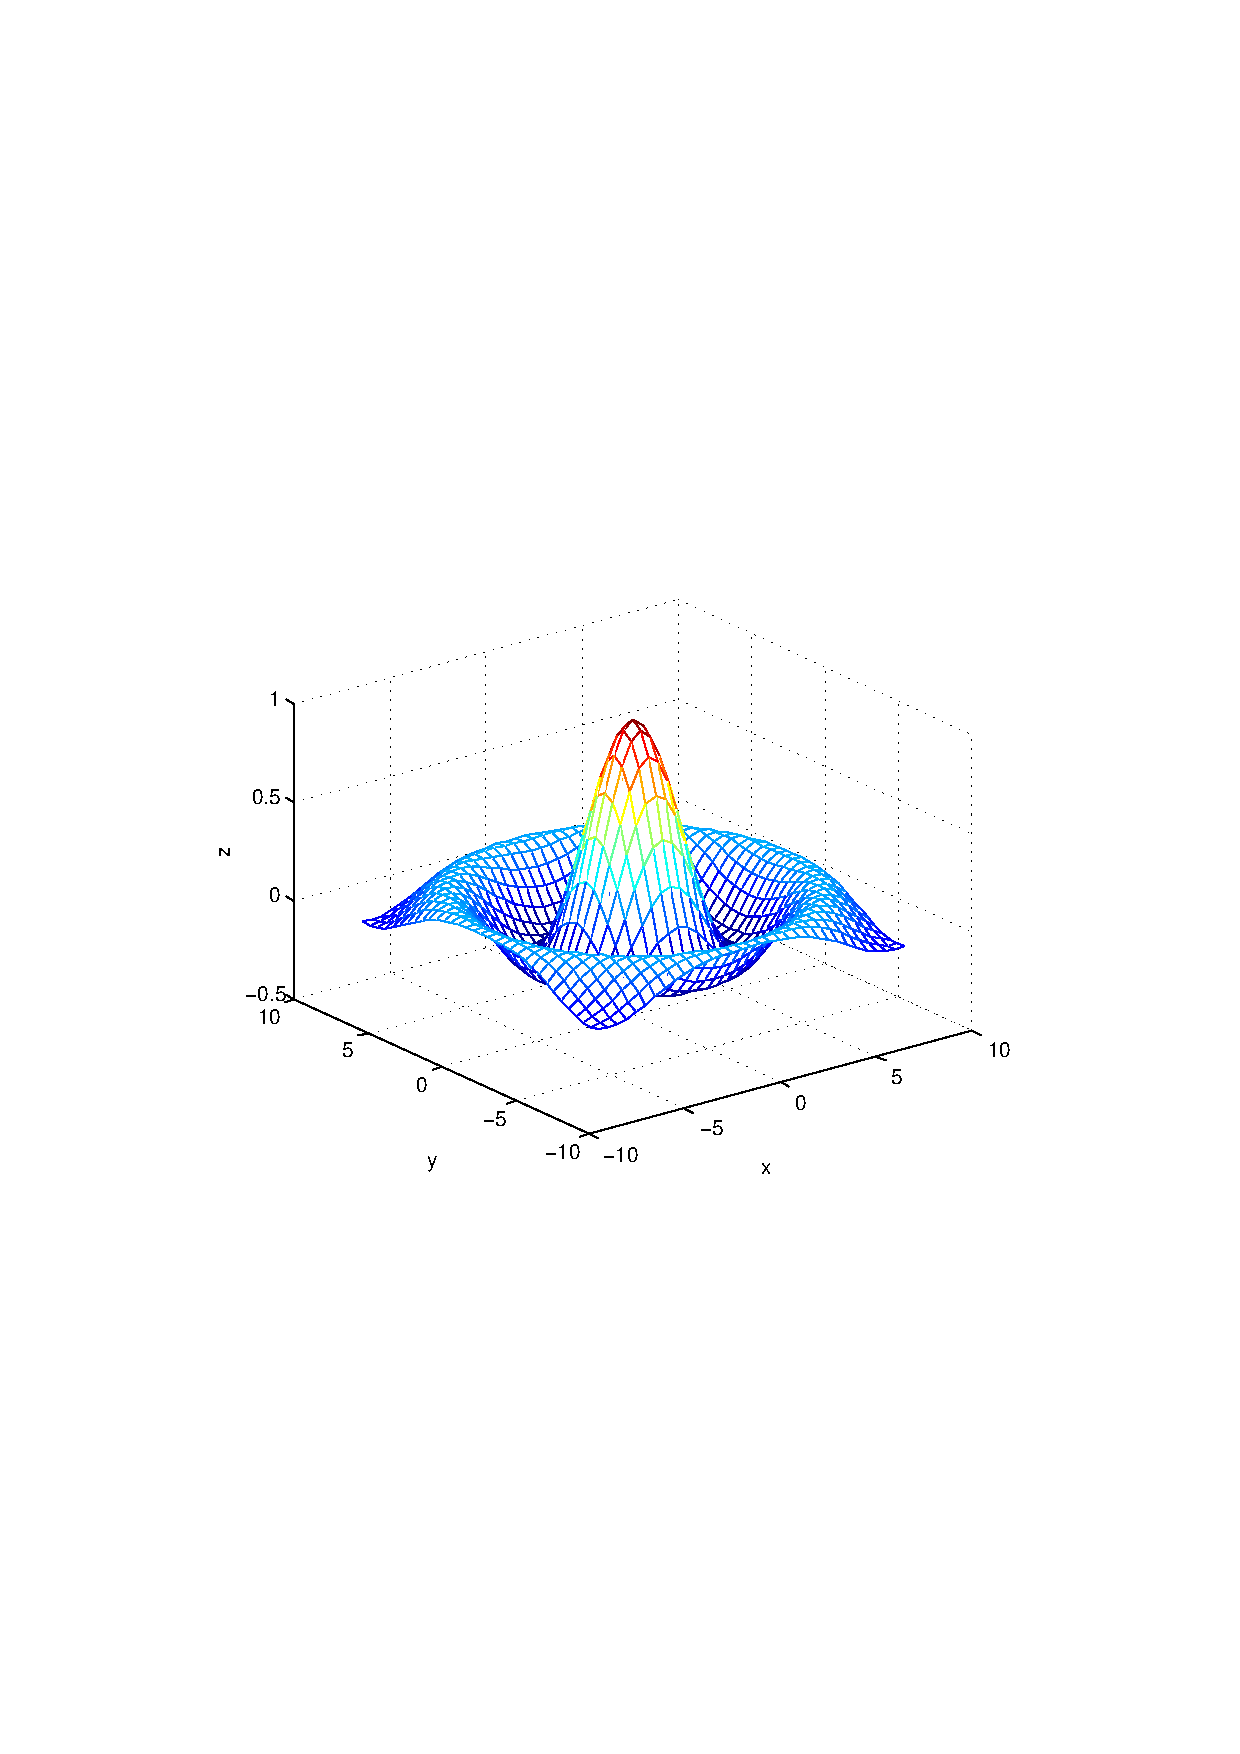
\includegraphics[width=12cm]{chapter4/img/sqrtsin.pdf}
% 		\label{fig:przyklad3D}
% 	\caption{Przykładowy wykres trójwymiarowy.}
% \end{figure}
% \newpage
% %-------------------------------------------------------------------------------------------------
% \begin{figure}[h!]
%   \centering
%   \subfloat[Wykres funkcji $\sin(x)$]{\label{fig:sinWyk}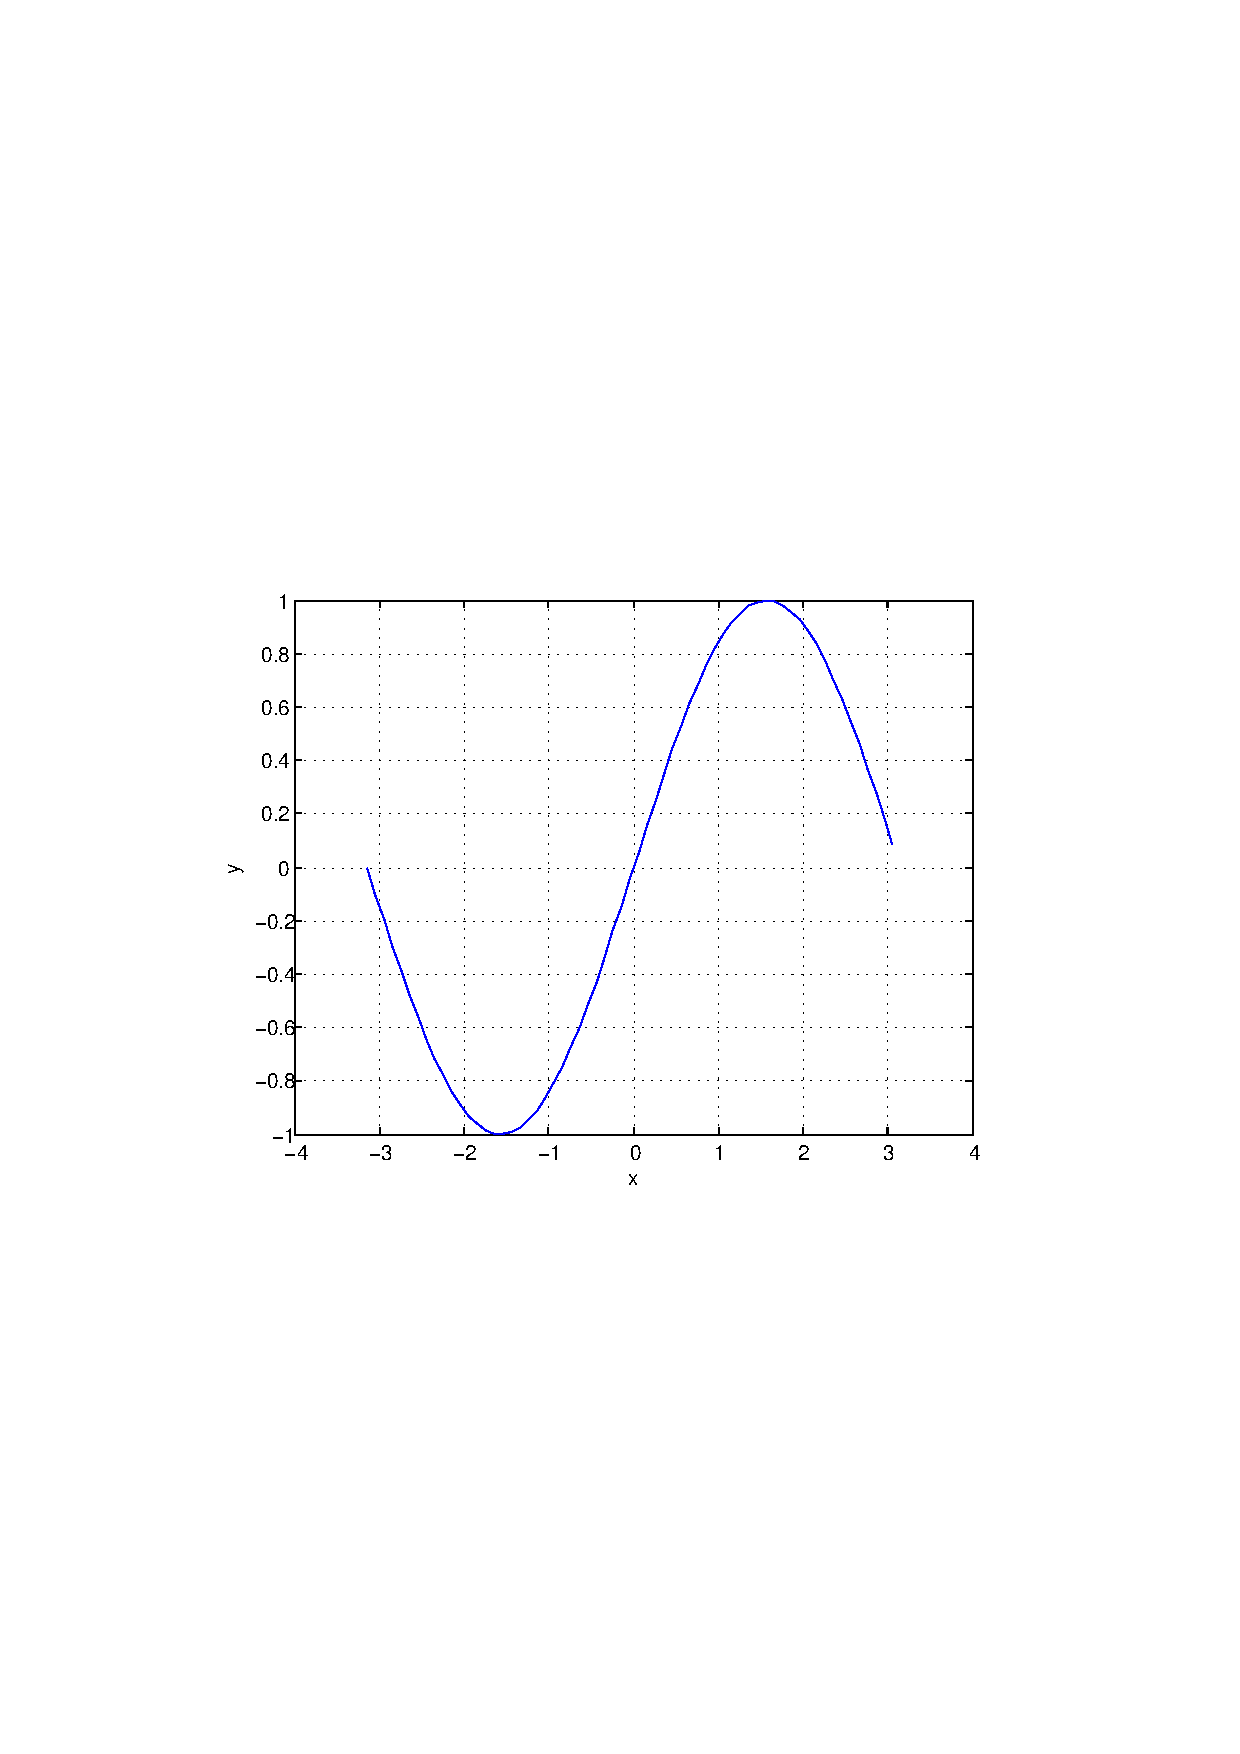
\includegraphics[width=0.45\textwidth]{chapter4/img/sin.pdf}}\quad
%   \subfloat[Wykres funkcji $\cos(x)$]{\label{fig:cosWyk}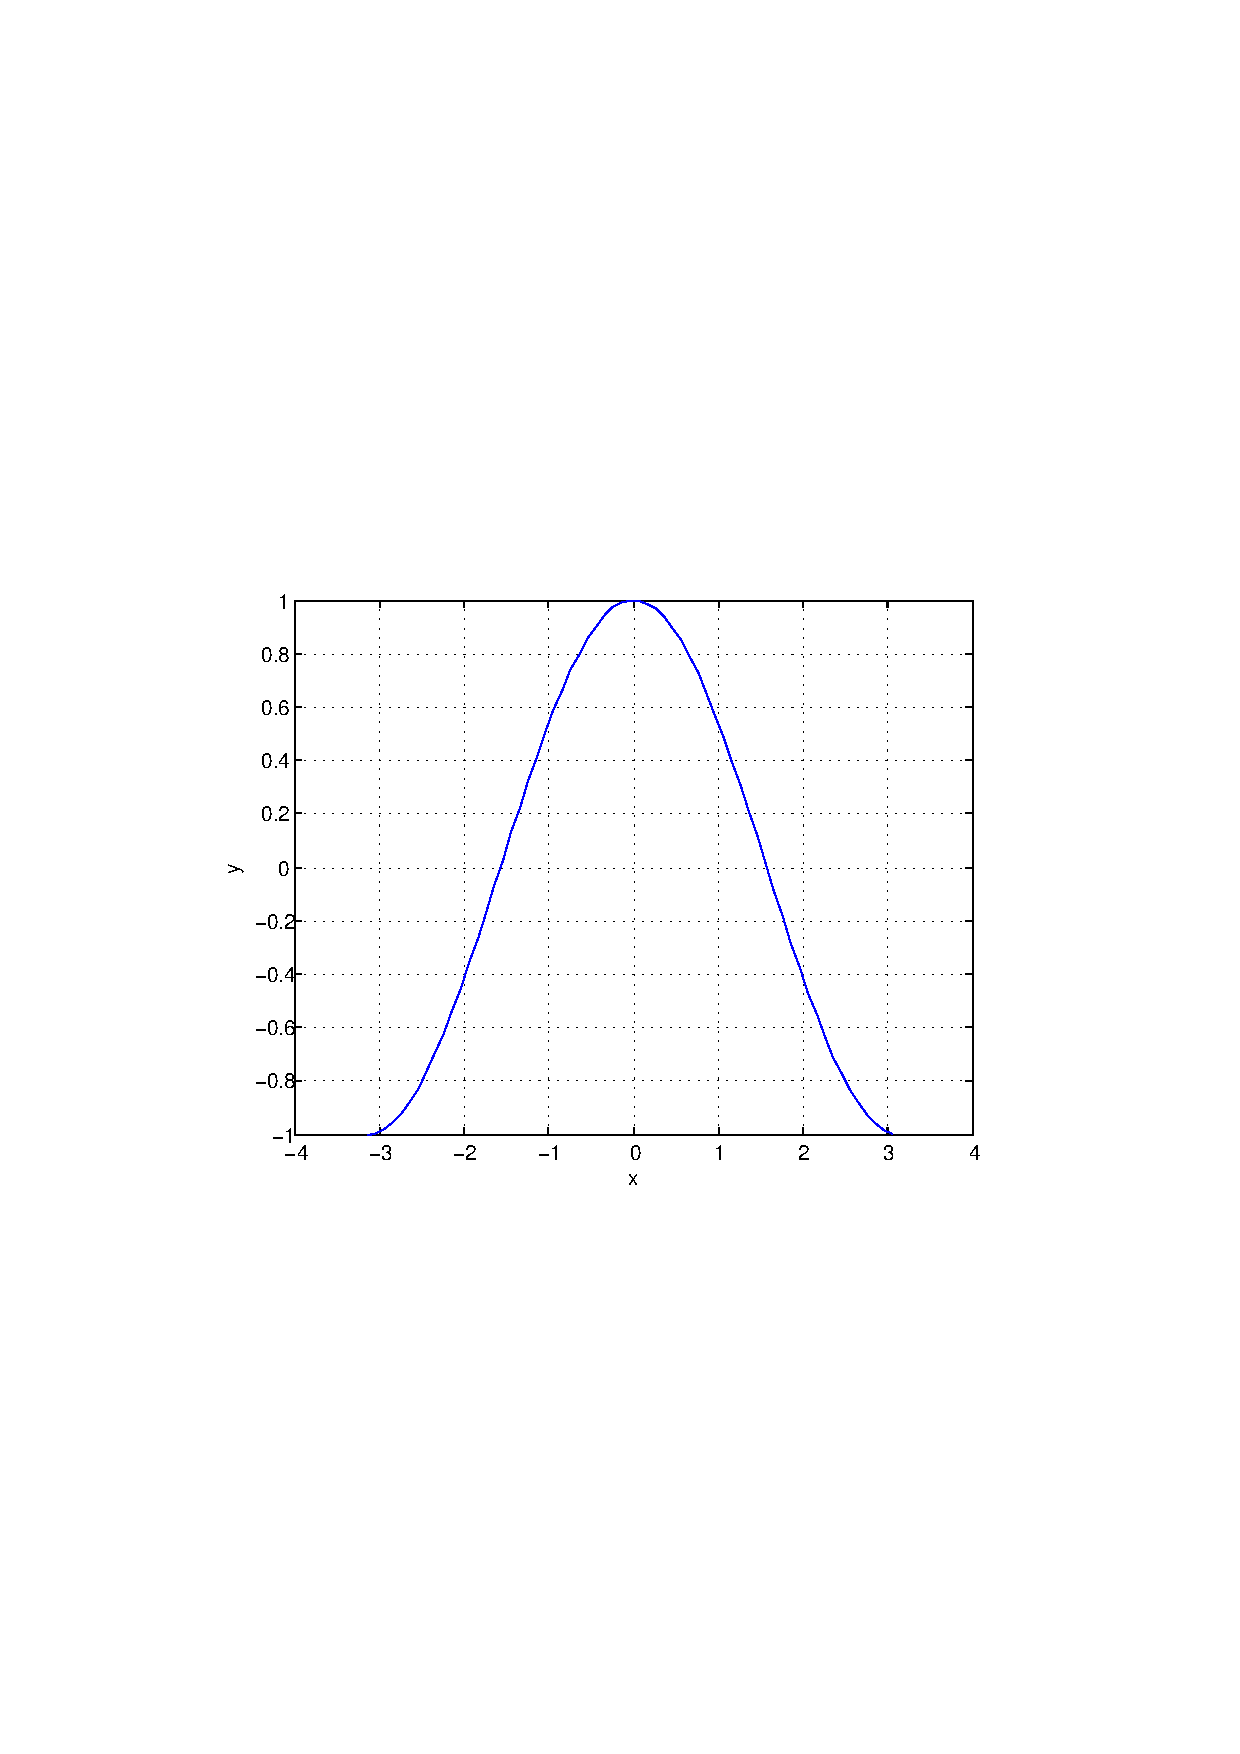
\includegraphics[width=0.45\textwidth]{chapter4/img/cos.pdf}}
%   \caption{Przykładowe wykresy funkcji $\sin (x)$ oraz $\cos (x)$ w przedziale $[-\pi, \pi]$.}
%   \label{fig:przyklad}
% \end{figure}

\chapter{Podsumowanie}
%=================================================================================================
Pracę powinien zakończyć rozdział podsumowujący rezultaty osiągnięte w pracy. Powinien obejmować co najmniej 3 strony, określając również w sposób jawny wnioski wynikające z przeprowadzonych badań. Każdy z nich musi opierać się o~materiał przedstawiony w głównej części pracy. Rozdział ten nie tylko dokonuje przeglądu rezultatów i~obserwacji, ale również je interpretuje. W wyniku dyskusji rezultatów powinno stać się jasnym, czy cele pracy sformułowane na początku zostały osiągnięte. Ważnym jest, aby wyjaśnić w~jakim stopniu otrzymane rezultaty uzasadniają osiągnięcie założonych celów. Należy również umiejscowić je w~kontekście prac innych osób zajmujących się podobnym zagadnieniem. Wskazane są elementy krytycyzmu co do otrzymanych rezultatów oraz podanie możliwości ich poprawy w~oparciu o~wiedzę zdobytą w~wyniku przygotowania pracy dyplomowej.


%========================================================================================
% Dodatki
%========================================================================================
% \begin{appendix}
% 	\appendix
% 	\chapter{Cel dodatków w pracy}
%=================================================================================================

Do materiałów, które mogą uzupełnić pracę, oprócz rysunków, tablic, ilustracji itp. należą także dodatki, nazwane również aneksami. Dają one możliwość albo dołączenia do tekstu głównego różnorodnego rodzaju informacji dodatkowych, albo wyłączenia z tekstu głównego tych wiadomości, które nie są w nim konieczne. Niekiedy pewne wiadomości wplecione w tekst niepotrzebnie go obciążają, przerywają zasadniczy wątek lub są nadmiernie szczegółowe. Jeśli mimo to wiadomości te są użyteczne i mogą być przydatne, warto oczyścić z nich tekst główny i zgrupować je na końcu pracy w postaci dodatków.


Przykładem użycia dodatków może być opis zawartości płyty CD lub DVD dołączonej do pracy lub instrukcje laboratoryjne stworzone w oparciu o napisaną pracę.

%=================================================================================================
% 	\chapter{Składanie wzorów}

W tej części nie opisywano już samych zasad tworzenia dokumentu, a zamiast tego skupiono się na przedstawieniu kilku przykładowo złożonych wzorów. W źródłach szablonu możliwe jest sprawdzenie jak wzór był pisany z wykorzystaniem notacji \LaTeX\ oraz pakietu \AmS. Więcej szczegółów zawiera rozdział ósmy świetnego opracowania \cite{companion:04} oraz dokumentacja pakietu \cite{ams:02}.
\begin{itemize}
\item Wzór dzielony i wyrównywany do znaku
\begin{equation}
	\begin{split}
		(a+b)^4  &= (a+b)^2 (a+b)^2 \\
					&= (a^2+2ab+b^2)(a^2+2ab+b^2) \\
					&= a^4+4a^3b+6a^2b^2+4ab^3+b^4. \\
	\end{split}
\end{equation}

\item Wzór w kilku liniach
\begin{multline}
	a+b+c+d+e+f+g+h+i+j+k+l+m+n\\
							o-p-r-s-t-u-w-x-y-z.
\end{multline}

\item Grupa wzorów
\begin{gather}
	a_1=b_1+c_1,\\
	a_2=b_2+c_2-d_2+e_2.
\end{gather}
\item Wzory z wyrównywaniem do znaku i osobną numeracją
\begin{align}
	x^2+y^2	&= 1, 					& x^3+y^3	&=1, \\
				x&=\sqrt{1-y^2},	& x 			&= \sqrt[3]{1-y^3}.
\end{align}

\begin{align}
	a_{11}& =b_{11},&
	a_{12}& =b_{12},\\
	a_{21}& =b_{21},&
	a_{22}& =b_{22}+c_{22}.
\end{align}
\item Wzory z wyrównywaniem do znaku oraz zewnętrznych marginesów i osobną numeracją 
\begin{flalign}
	a_{11}&	=b_{11},&
	a_{12}&	=b_{12},\\
	a_{21}&	=b_{21},&
	a_{22}&	=b_{22}+c_{22}.
\end{flalign}

\item Klamra
\begin{equation}
P_{r-j}=\begin{cases}
	0							& \text{jeśli $r-j$ jest nieparzyste},\\
	r!\,(-1)^{(r-j)/2}	& \text{w przeciwnym razie}.
\end{cases}
\end{equation}

\item Macierze
\begin{equation}
A=
	\begin{bmatrix}
		a	&	b	&	c		&	d	\\
		b	&	a	&	c+d	&	c-d	\\
		0	&	0	&	a+b	&	a-b	\\
		0	&	0	&	ab		&	cd	\\
	\end{bmatrix},
\end{equation}

\begin{equation}I_4=
	\begin{pmatrix}
			1 & 0 & 0 & 0 \\
		 	0 & 1 & 0 & 0 \\
			0 & 0 & 1 & 0 \\
			0 & 0 & 0 & 1 \\ 
	\end{pmatrix}
,\quad
\det{I_4}=
	\begin{vmatrix}
			1 & 0 & 0 & 0 \\
		 	0 & 1 & 0 & 0 \\
			0 & 0 & 1 & 0 \\
			0 & 0 & 0 & 1 \\ 
	\end{vmatrix}.
\end{equation}

\item Granica
\begin{equation}
\lim_{x\to 0}(1+x)^{\frac{1}{x}}=\mathrm{e}.
\end{equation}
\item Całka
\begin{equation}
\int_{0}^{1}3x^2\,\mathrm{d}x.
\end{equation}
\item Wzór z funkcjami trygonometrycznymi
\begin{equation}
\sin (\alpha \pm \beta) = \sin (\alpha) \cdot \cos (\beta) \pm \cos (\alpha) \cdot \sin (\beta).
\end{equation} 

\item Wzór Taylora
\begin{equation}
	\begin{split}f(x) &= f(a) + \frac{x-a}{1!} f^{(1)}(a) + \frac{(x-a)^2}{2!} f^{(2)}(a) + \ldots \\
							&+ \frac{(x-a)^n}{n!} f^{(n)}(a) + R_n(x,a)\\
							&= \sum\limits_{k=0}^n \left( \frac{(x-a)^k}{k!} f^{(k)}(a) \right) + R_n(x,a).
	\end{split}
\end{equation}
\end{itemize}
% \end{appendix}

%========================================================================================
% Literatura
%========================================================================================

\begin{flushleft}
	\bibliography{bibliography}
\end{flushleft}

\end{document}
%========================================================================================
% Koniec dokumentu
%========================================================================================